\section{Experiments}
\label{sec:experiments}

\subsection{Hyperparameter Selection}

\begin{figure}[htpb]
  \centering
  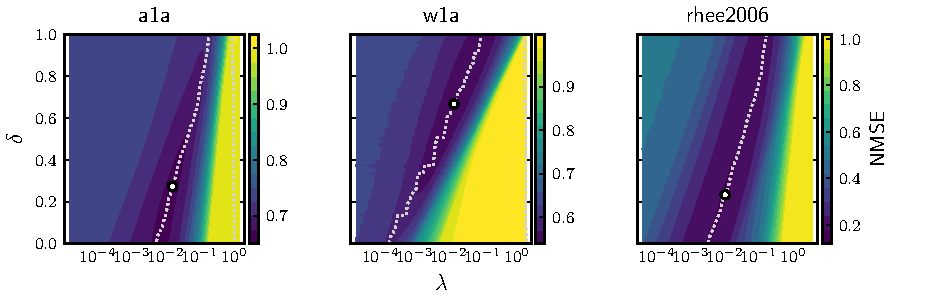
\includegraphics[]{plots/hyperopt.pdf}
  \caption{%
    Contour plots of hold-out error across a grid of \(\delta\) and \(\lambda\) values for the
    lasso.
  }
  \label{fig:hyperparameter selection}
\end{figure}

\subsection{Relative Size of Predictors in Model}

The next question we now ask ourselves is: given that both features are in the model, what are their respective sizes given differences in class balance (\(q\))?

To begin to answer this question, we conduct simulations on a two-dimensional problem. Along with our previous reasoning, we sample one feature from \(\normal(0, 0.5)\) and the other from \(\bernoulli(q)\), varying \(q\) in \([0.5, 0.99]\) to simulate the effect of class imbalance on the estimates from the model. We compare four different strategies of normalization:
\begin{description}
  \item[Mean-Std] Standardization
  \item[Mean-StdVar] Mean centering and scaling the normal feature by standard deviation and the binary feature by variance
  \item[Mean-Var] Mean centering and scaling each feature by its variance
  \item[None] No normalization
\end{description}

The results~(\Cref{fig:lasso-ridge-comparison}) show that when it comes to ridge, standardization creates class balance-insensitive estimates, whereas for the lasso, this is not the case. For the lasso, it is instead the Mean-StdVar and Mean-Var normalization methods that generate estimates that are insensitive to class imbalances.

\begin{figure}[htpb]
  \centering
  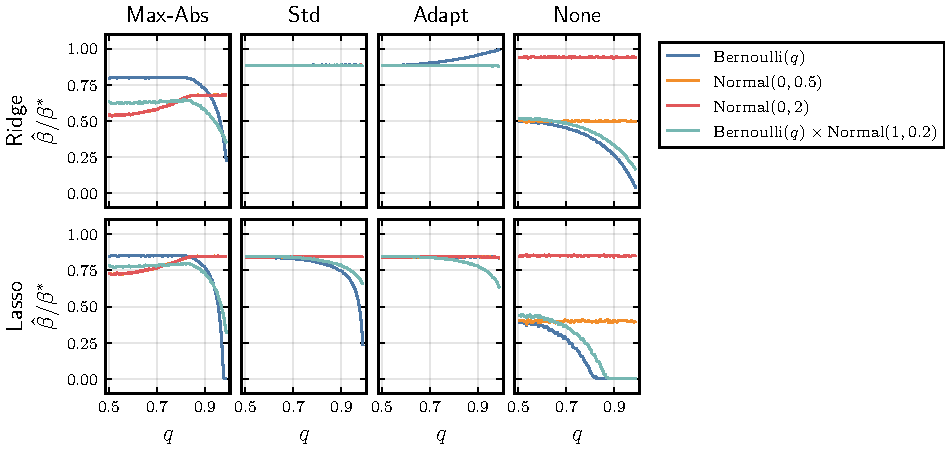
\includegraphics{plots/lassoridge_twodim.pdf}
  \caption{%
    Comparison between lasso and ridge estimators for a two-dimensional problem where one feature is generated from \(\bernoulli(q)\) and the other from \(\normal(0, 0.5)\) and the features are normalized in various ways.}
  \label{fig:lasso-ridge-comparison}
\end{figure}

\subsection{Varying Class Imbalances}

Here, we conduct an experiment on a \(300 \times 500\) design matrix, where the first 20 features are binary and the remaining ones are normally distributed with standard deviation 0.5. We consider four different cases for the class balances:
\begin{description}
  \item[Balanced] All of the signals have a class balance of 0.5.
  \item[Unbalanced] All of the signals have a class balance of 0.9.
  \item[Very Unbalanced] All of the signals have a class balance of 0.99.
  \item[Decreasing] The class balance of the signals decreases geometrically from 0.5 to 0.99.
\end{description}

To conduct the experiment, we generate random data and split it in a 50/50 training/test set split. Then, we select \(lambda\) using 10-fold cross validation on the training set and finally compute mean-squared error on the test set. We repeat this procedure 50 times for each combination of normalization type and class balance behavior.

The results~(\Cref{fig:binary-sim}) show that standardization performs best among the different types of normalization strategies.
% TODO: Expand on this.

\begin{figure}[htpb]
  \centering
  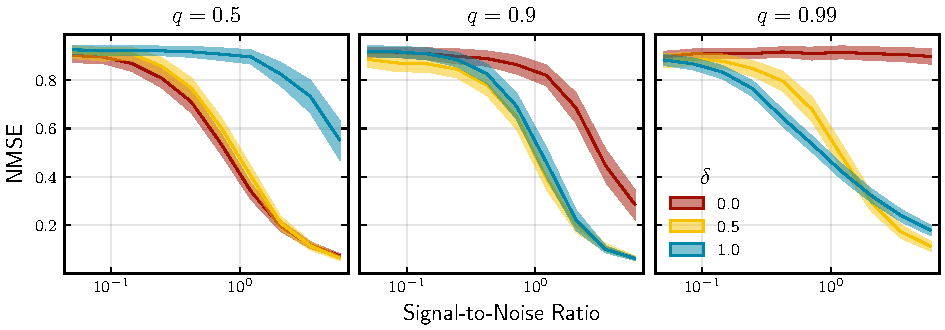
\includegraphics[]{plots/binary_data_sim.pdf}
  \caption{%
    Mean-squared error of \(y - \hat y\) for different types of normalizaion and types of class imbalances in a data set with only binary features.
  }
  \label{fig:binary-sim}
\end{figure}

\begin{figure}[htpb]
  \centering
  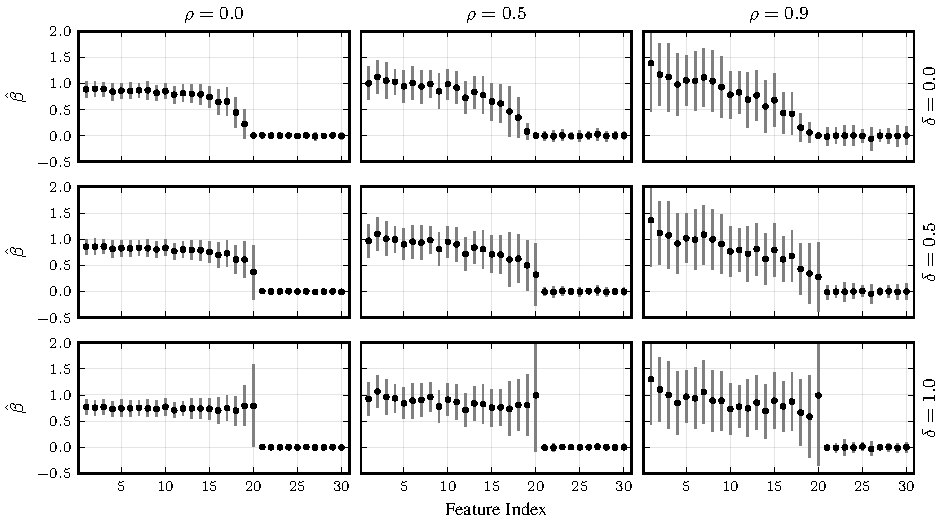
\includegraphics[]{plots/binary_decreasing.pdf}
  \caption{%
    Estimates of the regression coefficients, \(\hat{\vec{\beta}}\), for the first 40 coefficients in the experiment. All of the features are binary and the first 20 features correspond to true signals, with a geometrically decreasing class balance from 0.5 to 0.99. The remaining features have a class balance that's randomly sampled from a uniform distribution with parameters 0.5 and 0.99.}
  \label{fig:binary-decreasing}
\end{figure}

\begin{figure}[htpb]
  \centering
  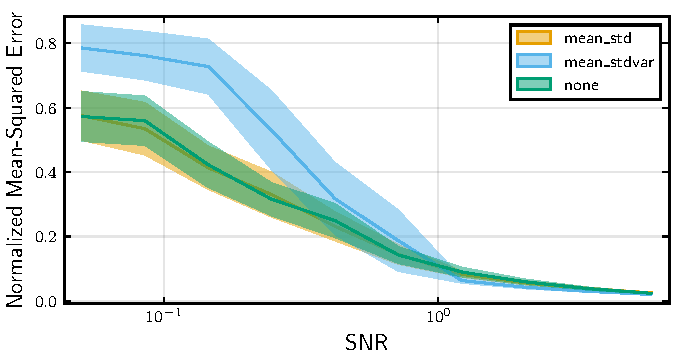
\includegraphics[]{plots/binary_decreasing_snr.pdf}
  \caption{%
    Prediction performance of an experiment with geometrically decreasing class balances for signals and varying signal to noise ratios.
  }
  \label{fig:binary-decreasing-snr}
\end{figure}

\subsection{Mixed Data}

\begin{figure}[htpb]
  \centering
  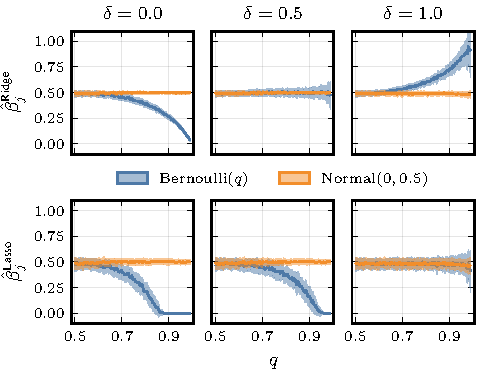
\includegraphics[]{plots/mixed_data.pdf}
  \caption{%
    An experiment with mixed (normal and Bernouli-distributed) data.
  }
  \label{fig:mixed-data}
\end{figure}
